\newpage
\hypertarget{TGGSchema}{}
\chapter{Creating your TGG schema}
\genHeader

Now that we have our source and target metamodels, we're going to start modeling the correspondence component of our envisioned triple language. 
This correspondence, or \emph{link metamodel},\define{Link \\ Metamodel} specifies \emph{correspondence types},\define{Correspondence Types} which will be used to connect specific elements of the source and target metamodels. 
These correspondence elements can also be thought of as \emph{traceability links}.
%
While the link metamodel is technically just a good old metamodel like any other, eMoflon provides a special wizard and project infrastructure (Eclipse nature, builder) for so-called \emph{integration projects}. 

The overall\define{TGG Schema} metamodel triple consisting of the relevant parts of the source, link, and target metamodels is called a \emph{TGG schema}.
%
A TGG schema can be viewed as the (metamodel) triple to which all \emph{new} triples must conform. 
In less technical lingo, it gives an abstract view on the relationships (correspondence) between two metamodels or domains. 
A domain expert should be able to understand why certain connected elements are related, irrespective of how the relationship is actually established by TGG rules, just by looking at the TGG schema. 

In our example schema, we will start by creating a link between our source \texttt{Box} and target \texttt{Dictionary} to express that these two container elements are related.

\begin{stepbystep}

\item Choose the \menuPath{Create new integration project} (\eMoflonCreateNewIntegrationProjectIcon) wizard from the eMoflon task bar, enter the project name as
\texttt{Learning\-Box\-To\-Dictionary\-In\-te\-gra\-tion}, and click \texttt{Finish} (\Cref{intgPackage}).

\item Open the schema file \texttt{src/org/moflon/tgg/mosl/Schema.tgg}, and import both repository projects by adding \moslTggCode{\#import} statements as depicted in \Cref{newSchema}.
As both projects are eMoflon projects (they don't \emph{have} to be but it makes things simpler), you can use a nifty little template provided by the editor for \menuPath{eMoflon imports}.
Just place your cursor at the beginning of the document and type \enquote{eMoflon}, then press \shortcut{Ctrl+Space} and confirm the suggestion with \shortcut{Enter}.
Repeat this procedure twice by entering \texttt{Dict\-io\-nary\-Lang\-uage} and \texttt{Lear\-ning\-Box\-Language}.

\item Now state which project is to be source (please choose \texttt{Learning\-Box\-Language}) and target (choose \texttt{Dictionary\-Language}) by stating the root packages in the \moslTggCode{#source} and \moslTggCode{#target} scopes of the schema (\Cref{newSchema}).
As with (almost) everything, the editor will try to help you with a reasonable selection if you hit \shortcut{Ctrl + Space}. 

\item Finally, create a first correspondence type named \texttt{BoxToDictionary} connecting \texttt{Box} and \texttt{Dictionary} as indicated in \Cref{newSchema}.
\end{stepbystep}

\begin{figure}[htbp]
\begin{center}
  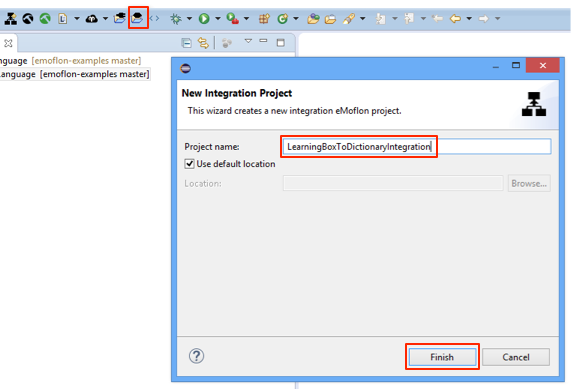
\includegraphics[width=\textwidth]{../../org.moflon.doc.handbook.04_tripleGraphTransformations/3_schema/newIntegrationProject}
  \caption{Create a new TGG integration project}  
  \label{intgPackage}
\end{center}
\end{figure}

\begin{figure}[htbp]
\begin{center}
  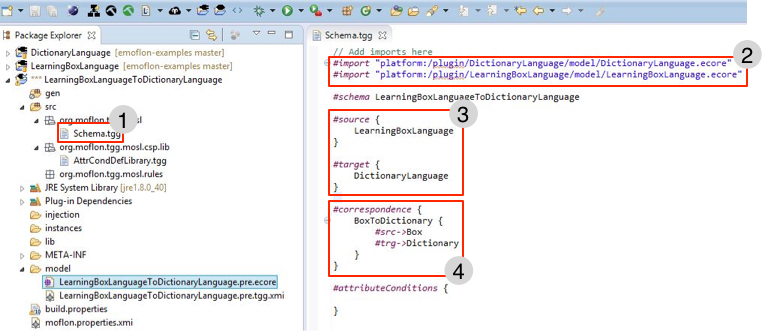
\includegraphics[width=\textwidth]{../../org.moflon.doc.handbook.04_tripleGraphTransformations/3_schema/newSchema}
  \caption{Add a first correspondence type (\texttt{BoxToDictionary})}  
  \label{newSchema}
\end{center}
\end{figure}
